\documentclass[a4paper,11pt]{article}
\usepackage{docmute}
\usepackage{import}
\usepackage{stmaryrd}
\usepackage{amsmath}
\usepackage{amsfonts}
\usepackage{simplebnf}
% \usepackage{caption}
\usepackage{subcaption}
\usepackage{CJKutf8}
\usepackage{booktabs}
\usepackage{semantic}
\usepackage{svg}
\usepackage[
    backend=biber,
    style=apa,
    natbib=true,
    doi=false,
    isbn=false,
    url=false,
]{biblatex}
\addbibresource{refs.bib}
\graphicspath{{figs/}}
\begin{document}
    \section{General repetition}

 % [General repetition]
    Patterns are ubiquitous across domains, arising from the repetition of invariance—whether explicit or abstract—among their instances. 
    From recognizing recurring architectural structures in cityscapes to identifying parallel syntactic forms in poetry, humans effortlessly detect and utilize patterns despite variations in their individual elements. This capacity extends to diverse domains: we discern shared narrative structures across novels, films, and music, and we uncover universal laws governing phenomena as distinct as ocean currents and atmospheric dynamics.  
    Moreover, humans can abstract patterns of patterns, as seen in the application of category theory to mathematics and programming.
    These examples illustrate our remarkable ability to not only detect abstract repetitions but also to productively employ them in navigating both the physical and mental worlds.
    Such capacity is believed to be a fundamental aspect of human cognition \parencite{pomiechowska2024compositionality}.

    % Here, we focus on patterns that arise from the repetition of hierarchical relations within sequential data, which we term \emph{structural repeats}. Unlike surface-level repetitions, structural repeats are not directly observable in the sequence itself but are inferable from the underlying generative process. Fig \ref{fig: examples of structural repeat} illustrates examples of structural repeats across diverse domains, including poetry, action planning, and music. Despite surface-level differences in the sequences, humans can perceive and appreciate the repetition of their underlying ``logic.''
    
    \begin{figure}
        \centering
        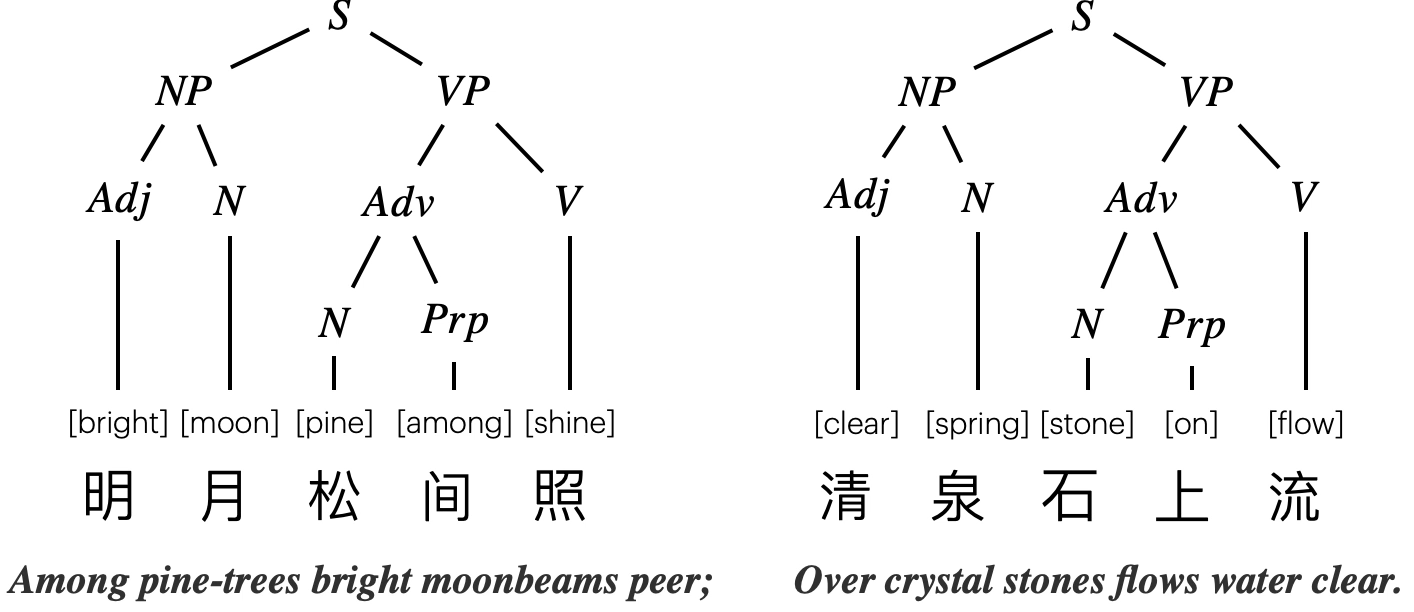
\includegraphics[width=0.9\linewidth]{figs/Chinese poem.png} 
        
        \caption{
        % A poetry written by Wang Wei (699–761 during Tang dynasty), translated by Xu Yuanchong, exhibiting parallel syntactic structure. 
        % %Such kind of parallel is not an incident but almost a requirement in Tang poetry, which support human's ability the both recognize and generalize such patterns.
        }
        \label{fig:poetry}
        
    \end{figure}

    \begin{figure}
        \centering
        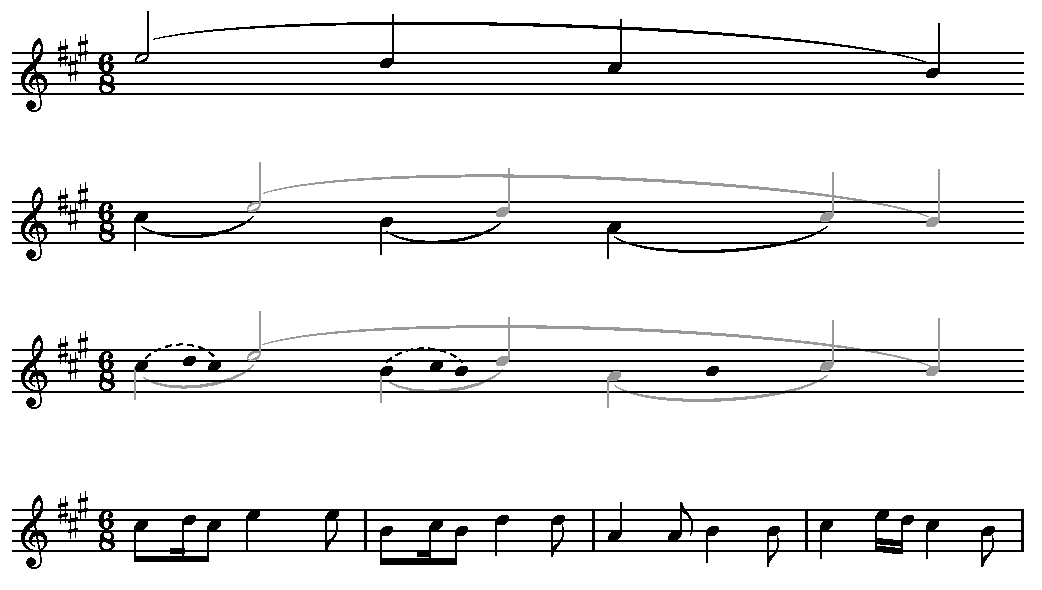
\includegraphics[width=0.9\linewidth]{K331Reduction.pdf}
        \caption{
        % A melodic reduction of K331 mm. 1-4. 
        % % Although no repetitions are evident on the musical surface, one might still hear a succession of ascending parallel thirds. The top-down derivation  reveals the notes $\hat{5}-\hat{4}-\hat{3}$ are first elaborated in the same way using ascending thirds. This parallel construction changes when the first two bars are further elaborated using neighboring motion whereas the third bar uses a passing motion.
        }
        \label{fig:music}
    \end{figure}
    \begin{figure}
        \centering
        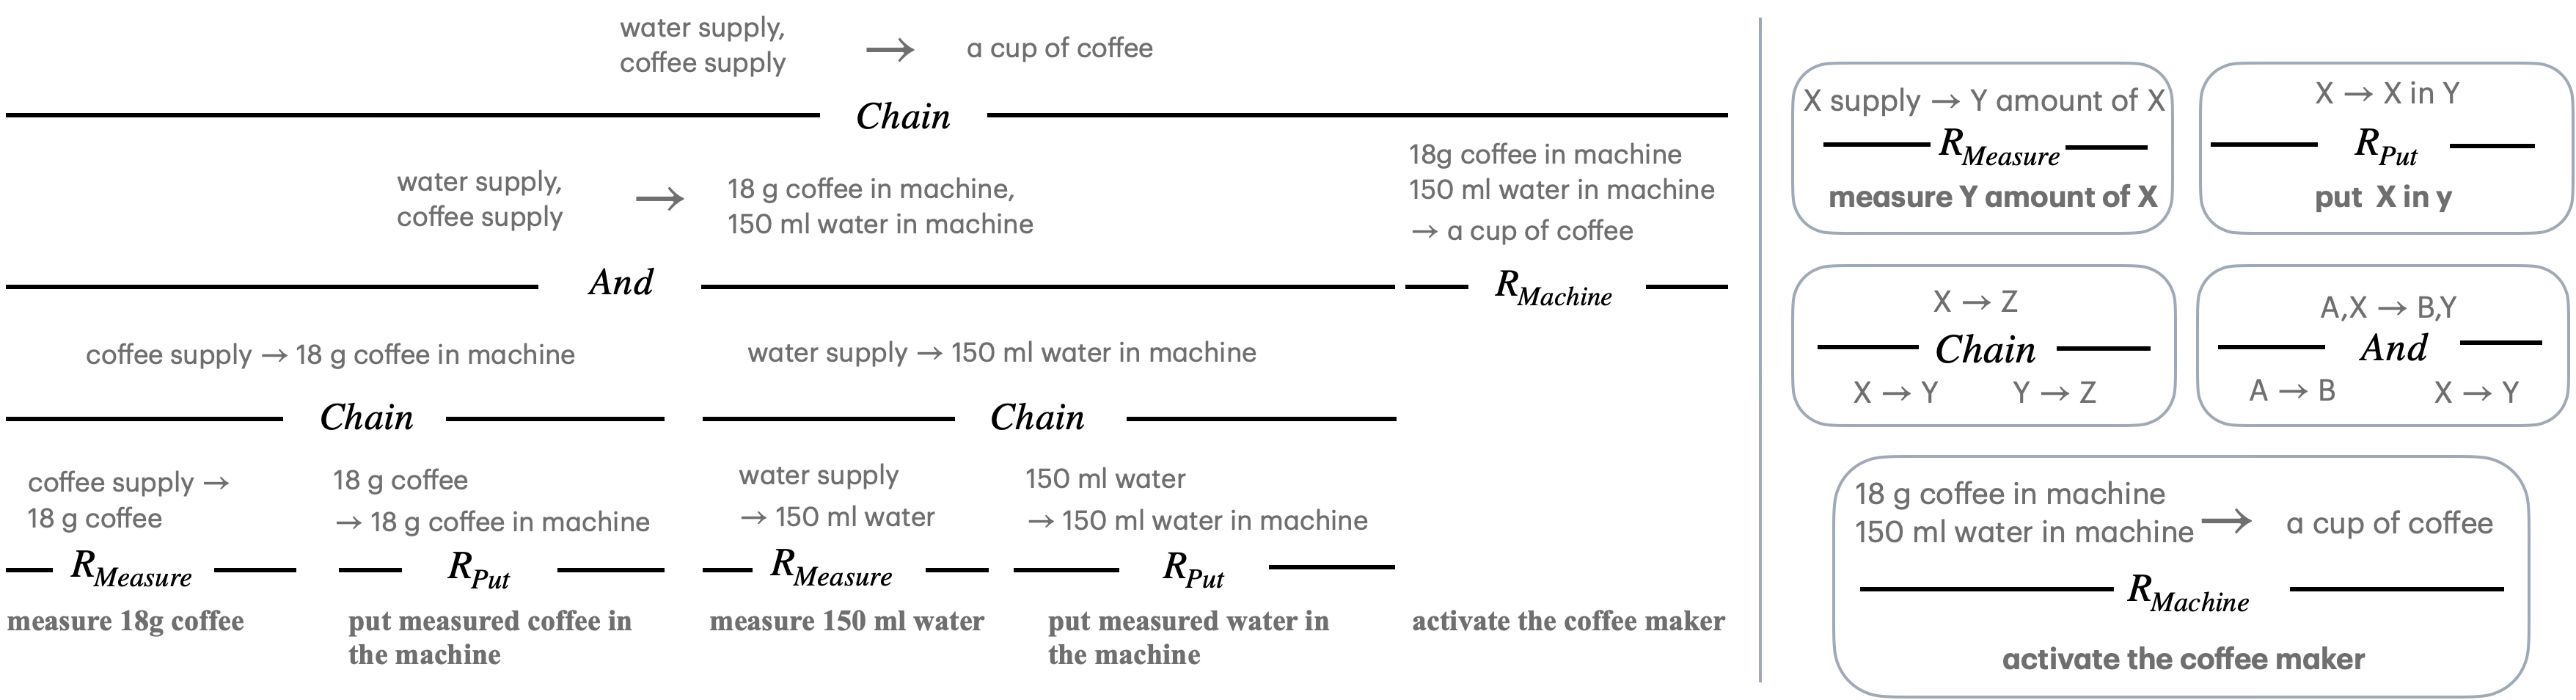
\includegraphics[width=1\linewidth]{coffee with rules.png} 
        \caption{
        % The hierarchical action planning involved in making coffee. 
        % % The leaves of the tree correspond to the observed actions involved in the process of making coffee. The internal nodes (colored text) show the tasks (e.g. the top-level task encodes how to obtain a cup of coffee from water and coffee supply). Relations (written on top of horizontal bars) show the decompositions of complex tasks into sub-tasks or concrete actions. This planning structure reveals latent repetition of the sub-computation $Chain \circ (R_{Measure} \otimes R_{Put})$. 
        % % The right figure lists the (polymorphic) primitive relations involved in the this planning process. 
        % % The $Chain$ relation combines tasks that must be carried out in order because one need the outcome of another. The $And$ relation combines tasks that must be both accomplished but the order is irrelevant.
        }
        \label{fig:coffee}
        % \caption{Three examples of structural repetition across domains demonstrates the kinds of computation involved in structural repeat. (\ref{fig:poetry}) An excerpt from the Tang poetry ``\begin{CJK*}{UTF8}{gbsn}\text{山居秋暝}\end{CJK*}'' written by Wang Wei (699–761), translated by Xu Yuanchong, exhibits parallel syntactic structure (repetition of complete computation). (\ref{fig:music}) A melodic reduction of the opening theme in K331 (mm. 1-4) shows mm. 1-3 share the same underlying generative process up to a certain point (repetition of suspended computation). (\ref{fig:coffee}) The hierarchical action planning involved in making coffee reveals polymorphic relations as the basis of structural repeats.}
    \end{figure}
    
    % How do humans infer the repetition of abstract patterns? Computational modeling in cognitive science serves as an important means to such questions by providing explicit and testable mechanisms for how the mind processes information \parencite{lake2017building, gershman2015computational, sun2009theoretical, sun2005levels}. In particular, generative models have been widely used to study sequences usually in form of (probabilistic) context-free grammar \parencite{jelinek1992basic}. Recent advances in program induction have further highlighted the connection between learning and the inference of generative programs that produce observed outputs \parencite{chater2013programs, lake2015human}, as emphasized in the 2018 CogSci workshop on ``Learning as Program Induction'' \parencite{Bramley2018Induction}. Building on these approaches, we study structural repeats using program induction methodologies guided by the principle of minimal description length \parencite{grunwald2007minimum}.
  
    % Our work adopts the following strategy: we first analyze the properties of mental processes involved in pattern recognition and use these insights to derive a mathematical model—a mini-programming language—that defines a hypothesis space of programs capable of generating observed sequences.
    % Following the idea of ``learning as program induction,'' we develop a weighted deduction algorithm \parencite{pereira1987prolog, sikkel1997parsing, shieber1995principles, nederhof2003weighted, Jason2023time} to infer programs that evaluate to the observed sequence.
    % While many candidate programs can produce the same output, humans do not consider all possibilities equally plausible. To address this, we use Minimum Description Length (MDL) \parencite{grunwald2007minimum} as a guiding principle to rank and disambiguate among programs, favoring those that offer the most compact representations.
    % Finally, we assess the plausibility of the minimal program. 
    % Our computational model, together with its implementation, provides a candidate theory and explicit descriptions on how the human minds recognize and process abstract relational repeats in sequential data.
  
% \subsection{Characterizing structural repetition}
    The examples of poetry (Fig.\ref{fig:poetry}), music (Fig.\ref{fig:music}), and hierarchical planning (Fig.\ref{fig:coffee}), progressively illustrate the complexities of structural repetition and the computational mechanisms required to process them.
    In poetry, parallel syntactic structures demand a hierarchical interpretation of sequences and the ability to identify the repeated substructures, such as derivation trees. 
    In the musical example, repeated computations can involve incomplete structures or ``holes,'' where repetitions are not exact subtrees but partial ones. 
    % while no repetitions are evident on the musical surface, one might still perceive a succession of ascending parallel thirds. 
    A top-down derivation reveals that notes $\hat{5}-\hat{4}-\hat{3}$ are first elaborated in the same way using ascending thirds (second row in Fig.\ref{fig:music}). This parallel construction then changes when the first two bars are further elaborated using neighboring motion whereas the third bar uses a passing motion (third row). 
    % This concept can be formalized as: the observations $y_1$ and $y_2$ contain structural repeat if there exists an incomplete computation $f$ and inputs $x_1,x_2$ such that $y_1 = f(x_1), y_2 = f(x_2)$. 
    Fig.\ref{fig:coffee} presents a hierarchical planning of actions involved in the task of making a cup of coffee from its ingredients. Notice that the actions involving preparing coffee ground and preparing water are ``repeated'' not in the literal sense but in terms of the relational structure of the underlying tasks. This example highlights the role of relations as the basic repeating units, emphasizing the repetition of computational processes (e.g., polymorphic production rules) rather than the input/output states of the computation (e.g., (non)terminals symbols).

    To summarize, we characterize structural repetition of hierarchical relations by two key properties. First, a single relation can manifest in multiple forms, similar to logical clauses involving meta-variables. Second, these relations can be inductively constructed via composition and duplications. Such construction process further entails the ability to express (a) incomplete/suspended computations and (b) various ways to repeat (the bindings of function variables in a composition expression).

    %cite : Thomas L. Griffiths, Joshua B. Tenenbaum, Tomer Ullman,Noah D. Goodman
\end{document}